\chapter{Darstellung der Ergebnisse}
\label{c:Ergebnisse}

\section{Daten zum Flugversuch der DO-128}

\subsection{Auftriebsbeiwert $\mathrm{C}_{\mathrm{A}}$ über Widerstandsbeiwert $\mathrm{C}_{\mathrm{W}}$}

\begin{figure}[H]
	\centering	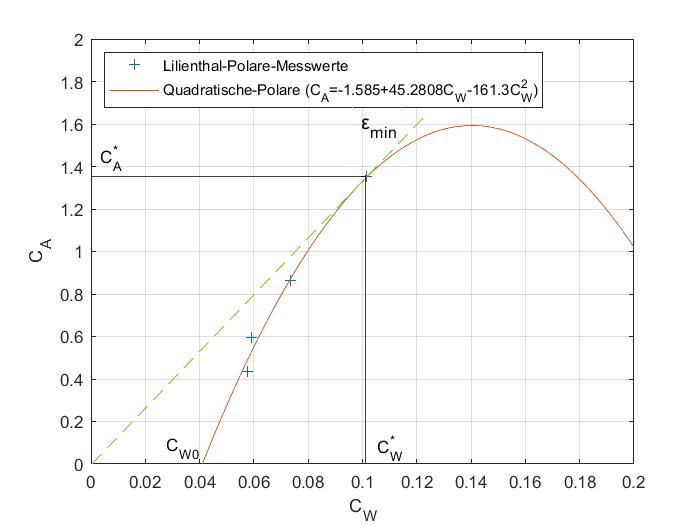
\includegraphics[width=0.7\textwidth]{./Bilder/CA_CW_fertig.jpg}
	\caption{$\mathrm{C}_{\mathrm{A}}$ über $\mathrm{C}_{\mathrm{W}}$ der DO-128}
	\label{fig:CA_CW_DO128}
\end{figure}

\subsection{Widerstand $\mathrm{W}$ über Fluggeschwindigkeit $\mathrm{V}$}

\begin{figure}[H]
	\centering	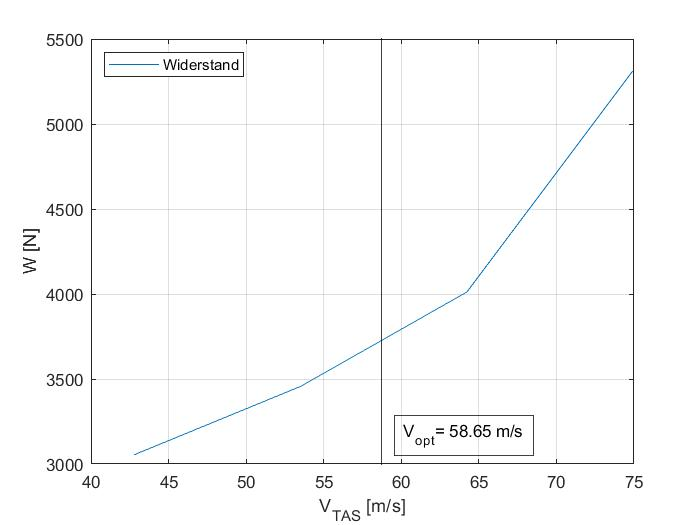
\includegraphics[width=0.7\textwidth]{./Bilder/W_uber_V.jpg}
	\caption{$\mathrm{W}$ über $\mathrm{V}$ der DO-128}
	\label{fig:W_V_DO128}
\end{figure}

\section{Daten zum Flugversuch der DO-28}

\subsection{Anstellwinkel $\alpha$ über Bahnneigungswinkel $\eta$}

\begin{figure}[H]
	\centering	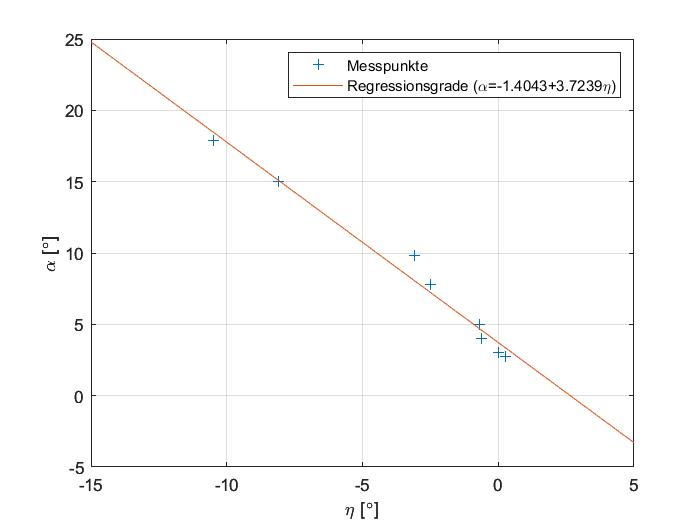
\includegraphics[width=0.7\textwidth]{./Bilder/alpha_eta_plot.jpg}
	\caption{$\alpha$ über $\eta$ der DO-28}
	\label{fig:alpha_eta_DO28}
\end{figure}

\subsection{Auftriebsbeiwert $\mathrm{C}_{\mathrm{A}}$ über Anstellwinkel $\alpha$}

\begin{figure}[H]
	\centering	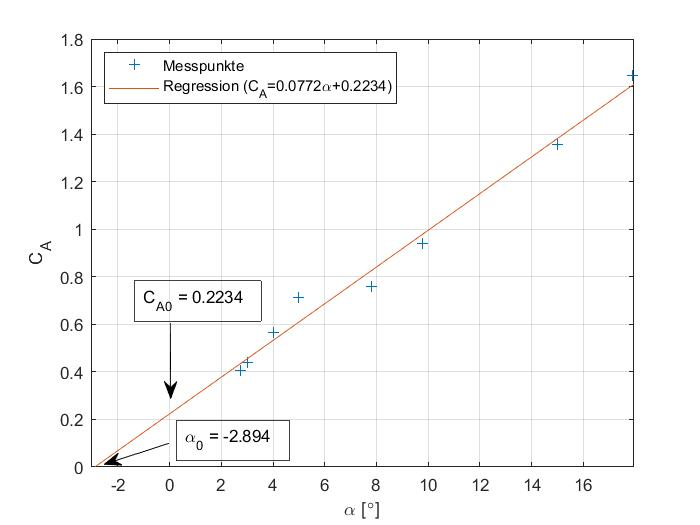
\includegraphics[width=0.7\textwidth]{./Bilder/CA_alpha_plot.jpg}
	\caption{$\mathrm{C}_{\mathrm{A}}$ über $\alpha$ der DO-28}
	\label{fig:CA_alpha_DO28}
\end{figure}

\subsection{Auftriebsbeiwert $\mathrm{C}_{\mathrm{A}}$ über Widerstandsbeiwert $\mathrm{C}_{\mathrm{W}}$}

\begin{figure}[H]
	\centering	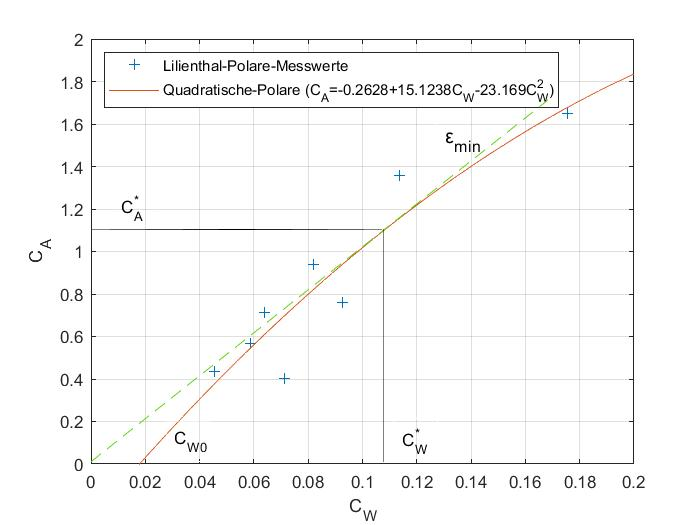
\includegraphics[width=0.7\textwidth]{./Bilder/CA_CW_DO28.jpg}
	\caption{$\mathrm{C}_{\mathrm{A}}$ über $\mathrm{C}_{\mathrm{W}}$ der DO-28}
	\label{fig:CA_CW_DO28}
\end{figure}

\subsection{Widerstand $\mathrm{W}$ über Fluggeschwindigkeit $\mathrm{V}$}

\begin{figure}[H]
	\centering	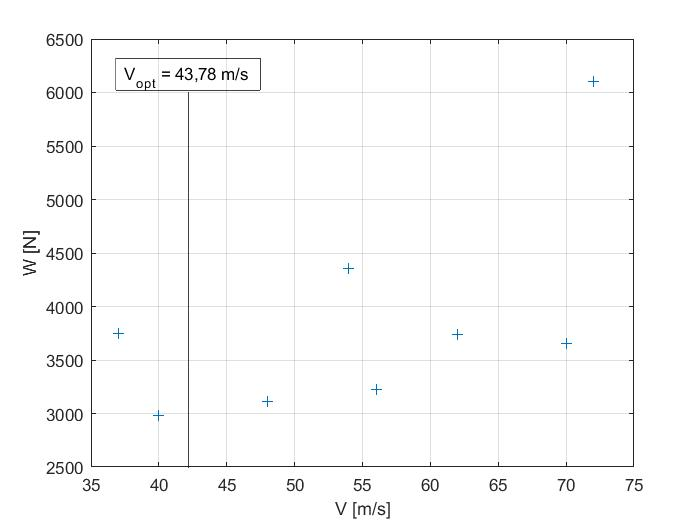
\includegraphics[width=0.7\textwidth]{./Bilder/W_V_DO28.jpg}
	\caption{$\mathrm{W}$ über $\mathrm{V}$ der DO-28}
	\label{fig:W_V_DO28}
\end{figure}


\subsection{Fluggeschwindigkeit $\mathrm{V}$ und Staudruck $\mathrm{q}$ über Anstellwinkel $\alpha$}

\begin{figure}[H]
	\centering	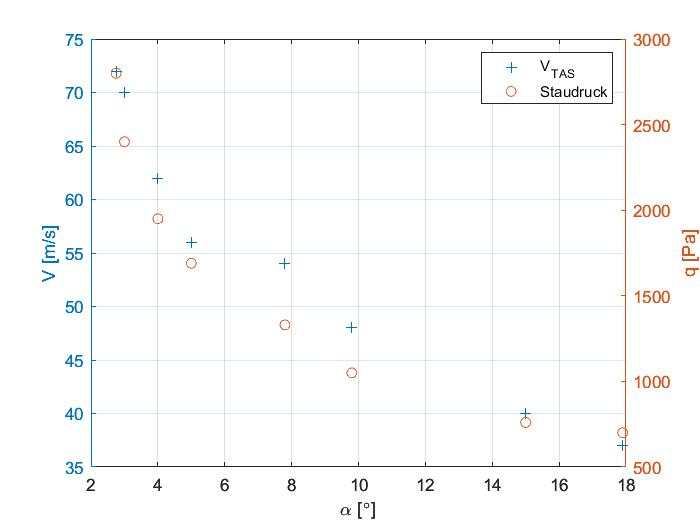
\includegraphics[width=0.7\textwidth]{./Bilder/V_q_alpha.jpg}
	\caption{$\mathrm{V}$ und $\mathrm{q}$ über $\alpha$ der DO-28}
	\label{fig:V_q_alpha_DO28}
\end{figure}